\documentclass{article}
\usepackage[brazil]{babel}
\usepackage{abstract}
\usepackage{tabularx}
\usepackage{tikz-er2}
\usetikzlibrary{positioning}
\usetikzlibrary{shadows}
%\usepackage{pgfplots}
\usetikzlibrary{backgrounds}

\tikzstyle{every entity} = [top color=white, bottom color=white, draw=black, drop shadow]
\tikzstyle{every weak entity} = [drop shadow={shadow xshift=.7ex, shadow yshift=-.7ex}]
\tikzstyle{every attribute} = [top color=white, bottom color=white!20, draw=black, node distance=0.75cm, drop shadow]
\tikzstyle{every relationship} = [top color=white, bottom color=white!20, draw=black, drop shadow]
\tikzstyle{every isa} = [top color=white, bottom color=white!20, draw=white!50!white!100]

\usepackage{stackengine}
\usepackage{multirow}
\usepackage[margin=1in]{geometry}
\usepackage{ulem}
\usepackage[colorlinks = true,
            linkcolor = blue,
            urlcolor  = blue,
            citecolor = blue,
            anchorcolor = blue]{hyperref} %smarter cross-references, these options turn links blue

\usepackage[parfill]{parskip}
\setlength{\parskip}{5pt} %plus 1 minus 1}
\setlength{\parindent}{30pt}
\usepackage{titlesec}
\usepackage{fourier-orns}
\usepackage{pifont}
\usepackage{amssymb}
\usepackage{leipzig}
\usepackage{caption}
\usepackage{booktabs}
\usepackage{natbib}
\usepackage{db-techreport}
\usepackage[no-math]{fontspec}
\usepackage{libertine}
\usepackage{color, soul}
\usepackage[linguistics]{forest}

\forestset{
  nice nodes/.style={
    for tree={
      inner sep=0pt,
      fit=band,
    },
  },
  default preamble=nice nodes,
}

\usepackage{gb4e}

\makeatletter
\def\@maketitle{\parfillskip=0pt
\noindent {\Large \bfseries \color{black} \@title}  \\ \hrule \noindent \@author \hfill \@date \par \vskip 1cm
}

\usepackage{tikz}
\newcommand{\circled}[1]{\begin{tikzpicture}[baseline=(word.base)]
\node[draw, rounded corners, text height=8pt, text depth=2pt, inner sep=2pt, outer sep=0pt, use as bounding box] (word) {#1};
\end{tikzpicture}
}

\RequirePackage{leipzig}
\RequirePackage{xspace}
\xspaceaddexceptions{]\}}

\let\oldemptyset\emptyset
\let\emptyset\varnothing
\newcommand{\nothing}{$\emptyset$}

\newcommand{\1}{\rlap{$'$}\xspace}
\newcommand{\0}{\rlap{\textsuperscript{$ˆ{\circ}$}}\xspace}
\newcommand{\Lb}[1]{$\text{[}_{\text{#1}}$ } %A more convenient left bracket
\newcommand{\Rb}[1]{$\text{]}_{\text{#1}}$ } %A more convenient left bracket
\newcommand{\gap}{\underline{\hspace{1.2em}}}
\newcommand{\vP}{\emph{v}P}
\newcommand{\lilv}{\emph{v}}
\newcommand{\Abar}{A$'$-} %A more convenient A-bar notation
\newcommand{\ph}{$\varphi$\xspace} %A more convenient phi
\newcommand{\pro}{\emph{pro}\xspace}
\newcommand{\subs}[1]{\textsubscript{#1}} %A more convenient subscript
%\newcommand{\hd}{$^{\circ}$\xspace} %Symbol for printing head / degree symbol
\newcommand{\spells}{$\Longleftrightarrow$} %spellout arrow for morph spellout rules
\newcommand{\tr}[1]{\textit{t}\textsubscript{\textit{#1}}} %easy traces with subscript
\newcommand{\supers}[1]{\textsuperscript{#1}}

% Abbreviations for glossing, based on Leipzig
\newleipzig{hab}{hab}{habitual}
\newleipzig{rem}{rem}{remote}
\newleipzig{sm}{sm}{subject marker}
\newleipzig{t}{t}{tense}
\newleipzig{aa}{aa}{anti-agreement}
\newleipzig{pron}{pron}{pronoun}
\newleipzig{rec}{rec}{recent}
\newleipzig{om}{om}{object marker}
%\newleipzig{ipfv}{ipfv}{imperfective}
\newleipzig{asp}{asp}{aspect}
\newleipzig{lk}{lk}{linker}
\newleipzig{pcl}{pcl}{particle}
\newleipzig{stat}{stat}{stative}
\newleipzig{ints}{ints}{intensive}
\newleipzig{ascl}{ascl}{assertive subject clitic}
\newleipzig{nascl}{nascl}{non-assertive subject clitic}
\newleipzig{ta}{ta}{tense and/or aspect}
\newleipzig{assoc}{assoc}{associative marker}
\newleipzig{hon}{hon}{honorific}
%\newleipzig{whprt}{wh}{\wh particle}
\newleipzig{sa}{sa}{subject agreement}
\newleipzig{conj}{conj}{conjunction}
%\newleipzig{loc}{loc}{locative}
\newleipzig{expl}{expl}{expletive}
\newleipzig{rcm}{rcm}{reciprocal marker}
\newleipzig{pers}{pers}{persistive}

\usepackage{phonrule}
\usepackage{textgreek}

%\usepackage{metalogo}


\renewcommand{\abstractnamefont}{\normalfont\large\textsc}

\title{Projeto do Banco de Dados SAM (v1.0)}
\author{Wladmir Cardoso Brand\~ao}
\date{Mar\c{c}o 30, 2020}



\begin{document}

\maketitle

\begin{abstract}

O presente relat\'orio apresenta o projeto do banco de dados SAM (Sistema Acad\^emico de Matrícula). Especificamente, o relat\'orio apresenta o resultado das atividades de especifica\c{c}\~ao do minimundo, an\'alise de requisitos, projeto conceitual, projeto l\'ogico e projeto f\'isico do SAM vers\~ao 1.0 (v1.0). As informa\c{c}\~oes necess\'arias para a realiza\c{c}\~ao das atividades de modelagem foram coletadas a partir de especifica\c{c}\~oes textuais fornecidas pelo usu\'ario final. O banco de dados \textsc{SAM (v1.0)} foi concebido dentro do paradigma relacional utilizando como base o modelo relacional, sendo constitu\'ido por um conjunto de cinco entidades, cinco relacionamentos e uma m\'edia de quatro atributos por entidade. Al\'em disso, as entidades e relacionamentos conceituais deram origem a um esquema de implementa\c{c}\~ao composto por sete tabelas e sete restri\c{c}\~oes de integridade referencial entre elas. Fisicamente, o banco de dados \'e composto por sete arquivos indexados com \'indice em cada um dos campos correspondentes \`as chaves prim\'arias das tabelas de origem. Adicionalmente, existem \'indices para cada uma das chaves estrangeiras para acelerar o processamento de transa\c{c}\~oes sobre os arquivos.

\end{abstract}

\section{Introdu\c{c}\~ao}
\label{sec:intro}
Institui\c{c}\~oes de ensino precisam manter seus registros acad\^emicos organizados e atualizados a fim de dar suporte a alunos e professores na execu\c{c}\~ao de suas atividades de aprendizagem, ensino e pesquisa.
A escolha da abordagem de banco de dados utilizada para organiza\c{c}\~ao e manuten\c{c}\~ao desses registros acad\^emicos influencia a efetividade com que as atividades s\~ao desenvolvidas.
O objetivo do presente trabalho \'e propor um projeto de banco de dados para um sistema acad\^emico de matr\'icula que pode ser utilizado por diversas institui\c{c}\~oes de ensino para gerenciar seus processos de matr\'icula de alunos em cursos.
Particularmente, prop\~oe-se uma especifica\c{c}\~ao de minimundo, an\'alise de requisitos, projeto conceitual, projeto l\'ogico e projeto f\'isico do banco de dados SAM (Sistema Acad\^emico de Matrícula), que em sua vers\~ao 1.0 \'e concebido no paradigma relacional, utilizando como base o modelo relacional e podendo ser implementado em sistemas gerenciadores de banco de dados (SGBD) relacionais comerciais.

A Se\c{c}\~ao~\ref{sec:minimundo} apresenta a especifica\c{c}\~ao de minimundo do babco de dados, incluindo uma descri\c{c}\~ao textual das principais caracter\'isticas e restri\c{c}\~oes de dados.
A Se\c{c}\~ao~\ref{sec:projetoconceitual} apresenta o projeto conceitual do banco de dados, incluindo diagrama entidade-relacionamento (ER) que representa de forma gr\'afica as principais defini\c{c}\~oes conceituais, pr\'oximas \`a forma como os usu\'arios percebem o banco de dados.
A Se\c{c}\~ao~\ref{sec:projetologico} apresenta o projeto l\'ogico do banco de dados, incluindo diagrama relacional que representa de forma gr\'afica as principais defini\c{c}\~oes para implementa\c{c}\~ao do banco de dados dentro do paradigma relacional.
%A Se\c{c}\~ao~\ref{sec:projetofisico} apresenta o projeto f\'isico do banco de dados, incluindo defini\c{c}\~oes relacionadas \`a organiza\c{c}\~ao de arquivos, registros e \'indices.

\section{Especifica\c{c}\~ao do Minimundo}
\label{sec:minimundo}
Essa se\c{c}\~ao apresenta a descri\c{c}\~ao textual de minimundo do SAM (v1.0), um banco de dados para um sistema acad\^emico que gerencia a matrícula de alunos em cursos em institui\c{c}\~oes de ensino. Em particular, os cursos da instituição de ensino são categorizados por áreas de conhecimento, sendo que um curso obrigatoriamente pertence a uma área e uma área pode possuir vários cursos. Além disso, uma área pode ser integrada por outras áreas, sendo que uma área só pode ser integrante de uma única área. As áreas são identificadas por sua sigla e possuem um nome. Os cursos são identificados por sua sigla e possuem nome, custo e professores, compostos por CPF e nome.
Alunos são identificados pelo seu CPF e possuem nome, composto de primeiro nome e sobrenome, sexo e data de nascimento. Cada aluno pode se matricular em diversos cursos, sendo que em cada curso podemos ter diversos alunos matriculados, mas devemos conhecer a data e se o aluno pagou ou não a matrícula no curso.
Cada curso é composto por módulos, sendo que um módulo compõe apenas um curso e não existem módulos sem vínculo a algum curso. Cada módulo é identificado por sua sigla e possui um nome. Cada módulo é composto por tópicos, sendo que cada tópico só existe em função de um módulo. Um tópico potencialmente pode ser identificado por sua sigla e possui nome e horas (carga horária do tópico). As horas do curso são derivadas da totalização das horas dos tópicos que compõem os módulos dos cursos.

\subsection{Requisitos Funcionais}
\label{sec:requisitosfuncionais}
Diferentes grupos de usu\'arios demandar\~ao diferentes opera\c{c}\~oes de manipula\c{c}\~ao de dados sobre diferentes por\c{c}\~oes do banco de dados. O grupo \textsc{Secretaria} demandar\'a atualiza\c{c}\~ao e recupera\c{c}\~ao de dados sobre praticamente todas os elementos do banco de.dados, uma vez que esse grupo ser\'a o respons\'avel por manter os dados atualizados, dando suporte aos outros grupos. O grupo \textsc{Professor} demandar\'a consultas de recupera\c{c}\~ao de dados sobre suas aloca\c{c}\~oes a cursos. O grupo \textsc{Aluno} demandar\'a consultas para atualiza\c{c}\~ao de seus dados cadastrais e para manipula\c{c}\~ao de dados sobre suas matr\'iculas. O grupo \textsc{Ger\^encia} demandar\'a a recupera\c{c}\~ao de dados agrupados sobre matr\'icula e cursos, tais como carga hor\'aria, custo e aloca\c{c}\~oes de professores e alunos. O grupo \textsc{Geral} demandar\'a recupera\c{c}\~ao de dados sobre \'areas, cursos, m\'odulos e t\'opicos para tomada de decis\~ao sobre inscri\c{c}\~ao como aluno ou professor da institui\c{c}\~ao de.ensino.
A Tabela~\ref{tab:query} apresenta as principais consultas que cada grupo de usu\'arios demandar\'a ao sistema de banco de dados, bem como a frequ\^encia esperada de submiss\~ao (A para alta, M para média e B para baixa.

\begin{table}[!htb]
    \caption{Frequ\^encia esperada de consultas por grupo de usu\'ario}
	\begin{tabularx}{\textwidth}{p{0.65cm} m{11.0cm} p{1.75cm} c}
		\toprule
		\multicolumn{2}{l}{\textbf{Consulta}} &
		\textbf{Grupo} &
		\textbf{Frequ\^encia}  \\ \midrule
		Q001 & Visualizar os cursos em que est\'a alocado & \textsc{Professor} & M \\
		Q002 & Atualizar dados cadastrais & \textsc{Aluno} & B \\
		Q003 & Efetivar matr\'icula em cursos & \textsc{Aluno} & B \\
		Q004 & Alterar matr\'icula em cursos & \textsc{Aluno} & B \\
		Q005 & Recuperar os cursos, e cargas hor\'arias, em que est\'a matriculado & \textsc{Aluno} & M \\
		Q006 & Visualizar lista de cursos por \'area de conhecimento & \textsc{Geral} & A \\
		Q007 & Visualizar m\'odulos por curso & \textsc{Geral} & A \\
		Q008 & Visualizar t\'opicos por m\'odulo do curso & \textsc{Geral} & A \\
		Q009 & Visualizar lista de professores por curso & \textsc{Geral} & M \\
		Q010 & Atualizar \'areas de conhecimento & \textsc{Secretaria} & B \\
		Q011 & Atualizar cursos & \textsc{Secretaria} & A \\
		Q012 & Atualizar m\'odulos de cursos & \textsc{Secretaria} & M \\
		Q013 & Atualizar t\'opicos de m\'odulos de cursos & \textsc{Secretaria} & M \\
		Q014 & Atualizar dados cadastrais de professores & \textsc{Secretaria} & B \\
		Q015 & Visualizar o n\'umero total de cursos, sua carga hor\'aria e custo total por \'area de conhecimento & \textsc{Ger\^encia} & A \\
		Q016 & Visualizar para cada curso seu custo relativo (custo absoluto por carga hor\'aria) e o n\'umero de m\'odulos que o comp\~oe & \textsc{Ger\^encia} & B \\
		Q017 & Visualizar para cada módulo de curso, o número total de tópicos e a carga horária mínima, máxima, média e total & \textsc{Ger\^encia} & B \\
		Q018 & Visualizar por área a média de carga horária e custo de cursos & \textsc{Ger\^encia} & B \\
		Q019 & Visualizar cada área, seu respectivo número de nível e o número de áreas de nível imediatamente inferior & \textsc{Ger\^encia} & B \\
		Q020 & Visualizar, para cada área, o curso com maior carga horária, e sua respectiva carga & \textsc{Ger\^encia} & A \\
		Q021 & Visualizar, para cada área, seus cursos e suas respectivas cargas horárias e custos, para os cursos em que as cargas horárias sejam maiores que a média dos cursos da área & \textsc{Ger\^encia} & A \\
		Q022 & Visualizar o número de matrículas efetuadas, & \textsc{Ger\^encia} & A \\
		\bottomrule
	\end{tabularx}
    \label{tab:query}
\end{table}


%\subsection{Requisitos N\~ao-Funcionais}
%\label{sec:requisitosnaofuncionais}

\clearpage
\section{Projeto Conceitual}
\label{sec:projetoconceitual}
Essa se\c{c}\~ao apresenta o projeto conceitual do SAM (v1.0), descrevento as principais estruturas e restri\c{c}\~oes conceituais do nanco de dados. Particularmente, a Figura~\ref{fig:er} apresenta o diagrama entidade-relacionamento (ER) do modelo conceitual do SAM.

\begin{center}
\begin{figure}[!htb]
\scalebox{.85}{
\begin{tikzpicture}[node distance=1.0cm, every edge/.style={link}]

% ENTIDADE AREA
\node[entity] (area) {\'Area};
\node[attribute] (areasigla) [above left = of area] {\key{Sigla}} edge (area);
\node[attribute] (areanome) [below = of area] {Nome} edge (area);

% RELACIONAMENTO AREA-AREA
\node[relationship] (integra) [right=1cm of area] {integra} edge (area);
\draw [line width=0.35mm] (0.0,0.55) -- (0.0,1.75) -- (3.0, 1.75) -- (3.0,0.9);

% RELACIONAMENTO AREA-CURSO
\node[relationship] (areacurso) [left=2.5cm of area] {possui} edge (area);

% ENTIDADE CURSO
\node[entity] (curso) [below=2cm of areacurso] {Curso} edge [total] (areacurso);
\node[attribute] (cursosigla) [above left = of curso] {\key{Sigla}} edge (curso);
\node[attribute] (cursonome) [above right = of curso] {Nome} edge (curso);
\node[derived attribute] (cursohoras) [below = of curso] {Horas} edge (curso);
\node[attribute] (cursocusto) [below left = of curso] {Custo} edge (curso);
\node[multi attribute] (cursoprofessores) [below right = of curso] {Professores} edge (curso);
\node[attribute] (professoresCPF) [below = of cursoprofessores] {CPF} edge (cursoprofessores);
\node[attribute] (professoresnome) [below right = of cursoprofessores] {Nome} edge (cursoprofessores);

% RELACIONAMENTO CURSO-MODULO
\node[relationship] (cursomodulo) [right=1.5cm of curso] {possui} edge (curso);

% RELACIONAMENTO CURSO-ALUNO
\node[relationship] (cursoaluno) [left=2cm of curso] {matricula} edge (curso);
\node[attribute] (cursoalunodata) [above = of cursoaluno] {Data} edge (cursoaluno);
\node[attribute] (cursoalunopago) [above left = of cursoaluno] {Pago} edge (cursoaluno);

% ENTIDADE ALUNO
\node[entity] (aluno) [below=2.5cm of cursoaluno] {Aluno} edge (cursoaluno);
\node[attribute] (alunoCPF) [below left = of aluno] {\key{CPF}} edge (aluno);
\node[attribute] (alunonome) [below right = of aluno] {Nome} edge (aluno);
\node[attribute] (alunodata) [right = of aluno] {Data Nascimento} edge (aluno);
\node[attribute] (alunosexo) [below = of aluno] {Sexo} edge (aluno);
\node[attribute] (alunoprimeiro) [right = of alunonome] {Primeiro Nome} edge (alunonome);
\node[attribute] (alunosobrenome) [below right = of alunonome] {Sobrenome} edge (alunonome);

% ENTIDADE MODULO
\node[entity] (modulo) [right=1.5cm of cursomodulo] {M\'odulo} edge [total] (cursomodulo);
\node[attribute] (modulosigla) [above = of modulo] {\key{Sigla}} edge (modulo);
\node[attribute] (modulonome) [above right = of modulo] {Nome} edge (modulo);

% RELACIONAMENTO MODULO-TOPICO
\node[ident relationship] (modulotopico) [right=1.5cm of modulo] {possui} edge (modulo);

% ENTIDADE TOPICO
\node[weak entity] (topico) [below=1cm of modulotopico] {T\'opico} edge [total] (modulotopico);
\node[attribute] (topicosigla) [left = of topico] {\discriminator{Sigla}} edge (topico);
\node[attribute] (topiconome) [below left = of topico] {Nome} edge (topico);
\node[attribute] (topicohoras) [below = of topico] {Horas} edge (topico);

% CARDINALIDADE AREA-AREA
\draw[link] (area) |- node [pos=0.95, auto] {1} (integra);
\node at (2.8,1.1) {N};

% CARDINALIDADE AREA-CURSO
\draw[link] (areacurso) -- node [pos=0.05, auto] {1} (area);
\draw[link, draw=white] (areacurso) -- node [pos=0.1, auto] {N} (curso);

% CARDINALIDADE CURSO-MODULO
\draw[link] (curso) |- node [pos=0.95, auto] {1} (cursomodulo);
\draw[link, draw=white] (cursomodulo) -- node [pos=0.1, auto] {N} (modulo);

% CARDINALIDADE CURSO-ALUNO
\draw[link] (cursoaluno) -- node [pos=0.05, auto] {N} (curso);
\draw[link] (cursoaluno) -- node [pos=0.15, auto] {N} (aluno);

% CARDINALIDADE MODULO-TOPICO
\draw[link] (modulo) |- node [pos=0.95, auto] {1} (modulotopico);
\draw[link, draw=white] (topico) -- node [pos=0.85, auto] {N} (modulotopico);
\end{tikzpicture}
}
\caption{Diagrama ER do modelo conceitual do banco de dados SAM (v1.0)}
\label{fig:er}
\end{figure}
\end{center}

Adicionalmente, a Tabela~\ref{tab:er} apresenta com mais detalhes os elementos descritos no diagrama apresentados na Figura~\ref{fig:er}. Na Tabela~\ref{tab:er}, podemos observar que foram identificadas na descri\c{c}\~ao textual do minimundo cinco entidades, com uma m\'edia de quatro atributos por entidade. Al\'em disso, foram identificados cinco relacionamentos entre entidades, bem como suas respectivas restri\c{c}\~oes de cardinalidade, e tr\^es restri\c{c}\~oes de totalidade presentes em tr\^es relacionamentos diferentes.

\begin{table}[!htb]
    \caption{Elementos do modelo conceitual do banco de dados SAM (v1.0)}
	\begin{tabularx}{\textwidth}{p{2.25cm} m{2.0cm} c p{2.5cm} m{1.75cm} m{4.75cm}}
		\toprule
		\textbf{Tipo} &
		\textbf{Subtipo} &
		\textbf{ID} &
		\textbf{R\'otulo} &
		\textbf{Refer\^encia} &
		\textbf{Descri\c{c}\~ao} \\ \midrule
		Entidade & Forte & E001 & Aluno & & \\
		Entidade & Forte & E002 & \'Area & & \\
		Entidade & Forte & E003 & Curso & & \\
		Entidade & Forte & E004 & M\'odulo & & \\
		Entidade & Fraca & E005 & T\'opico & & \\
		Relacionamento & Forte & R001 & integra & E002 & \\
		Relacionamento & Forte & R002 & matricula & E001, E003 & \\
		Relacionamento & Forte & R003 & possui & E002, E003 & \\
		Relacionamento & Forte & R004 & possui & E003, E004 & \\
		Relacionamento & Fraco & R005 & possui & E004, E005 & \\
		Atributo & Chave & A001 & CPF & E001 & \\
		Atributo & Composto & A002 & Nome & E001 & \\
		Atributo & Simples & A003 & Primeiro Nome & E001, A002 & \\
		Atributo & Simples & A004 & Sobrenome & E001, A002 & \\
		Atributo & Simples & A005 & Sexo & E001 & \\
		Atributo & Simples & A006 & Data Nascimento & E001 & \\
		Atributo & Chave & A007 & Sigla & E002 & \\
		Atributo & Simples & A008 & Nome & E002 & \\
		Atributo & Chave& A009 & Sigla & E003 & \\
		Atributo & Simples & A010 & Nome & E003 & \\
		Atributo & Simples & A011 & Custo & E003 & \\
		Atributo & Derivado & A012 & Horas & E003 & \\
		Atributo & Multivalorado Composto & A013 & Professores & E003 & \\
		Atributo & Simples & A014 & CPF & E003, A013 & \\
		Atributo & Simples & A015 & Nome & E003, A013 & \\
		Atributo & Chave & A016 & Sigla & E004 & \\
		Atributo & Simples & A017 & Nome & E004 & \\
		Atributo & Chave & A018 & Sigla & E005 & \\
		Atributo & Simples & A019 & Nome & E005 & \\
		Atributo & Simples & A020 & Horas & E005 & \\
		Restri\c{c}\~ao & Totalidade & C001 & & R002 & E003 total em R002 \\
		Restri\c{c}\~ao & Totalidade & C002 & & R004 & E004 total em R004 \\
		Restri\c{c}\~ao & Totalidade & C003 & & R005 & E005 total em R005 \\
		Restri\c{c}\~ao & Cardinalidade & C004 & 1-N & R001 & E002 fun\c{c}\~ao \textit{integrado} (1), E002 fun\c{c}\~ao \textit{integrante} (N) \\
		Restri\c{c}\~ao & Cardinalidade & C005 & N-N & R002 & E003 fun\c{c}\~ao \textit{matriculante} (N), E001 fun\c{c}\~ao \textit{matriculado} (N) \\
		Restri\c{c}\~ao & Cardinalidade & C006 & 1-N & R003 & E002 fun\c{c}\~ao \textit{possuidor} (1), E003 fun\c{c}\~ao \textit{possu\'ido} (N) \\
		Restri\c{c}\~ao & Cardinalidade & C007 & 1-N & R004 & E003 fun\c{c}\~ao \textit{possuidor} (1), E004 fun\c{c}\~ao \textit{possu\'ido} (N) \\
		Restri\c{c}\~ao & Cardinalidade & C008 & 1-N & R005 & E004 fun\c{c}\~ao \textit{possuidor} (1), E005 fun\c{c}\~ao \textit{possu\'ido} (N) \\
		\bottomrule
	\end{tabularx}
    \label{tab:er}
\end{table}


\clearpage
\section{Projeto L\'ogico}
\label{sec:projetologico}
Essa se\c{c}\~ao apresenta o projeto l\'ogico do banco de dados SAM (v1.0), descrevento as principais estruturas e restri\c{c}\~oes l\'ogicas baseadas no modelo de implementa\c{c}\~ao relacional. Particularmente, a Figura~\ref{fig:eer} apresenta o diagrama relacional do banco de dados, mapeado a partir do modelo conceitual descrito na Se\c{c}\~ao~\ref{sec:projetoconceitual} do presente relat\'orio.

\begin{center}
\begin{figure}[!htb]
\scalebox{.98}{
\begin{tikzpicture}[transform shape]
% CURSO
\node at (0.15,1.3) {CURSO};
\filldraw[fill=black!10!white] (-0.5,0.2) rectangle (1.0,1.0) node[pos=.5] {\underline {Sigla}};
\filldraw[fill=black!10!white] (1.0,0.2) rectangle (2.5,1.0) node[pos=.5] {Nome};
\filldraw[fill=black!10!white] (2.5,0.2) rectangle (4.0,1.0) node[pos=.5] {Horas};
\filldraw[fill=black!10!white] (4.0,0.2) rectangle (5.5,1.0) node[pos=.5] {Custo};
\filldraw[fill=black!10!white] (5.5,0.2) rectangle (7.0,1.0) node[pos=.5] {Area};

% AREA
\node at (8.0,1.3) {AREA};
\filldraw[fill=black!10!white] (7.5,0.2) rectangle (9.0,1.0) node[pos=.5] {\underline {Sigla}};
\filldraw[fill=black!10!white] (9.0,0.2) rectangle (10.5,1.0) node[pos=.5] {Nome};
\filldraw[fill=black!10!white] (10.5,0.2) rectangle (13.0,1.0) node[pos=.5] {SuperArea};

% LINK AREA-AREA
\draw[-] (11.75, -0.25) -- (11.75, 0.2);
\draw[->] (8.5, -0.25) -- (8.5, 0.2);
\draw (8.5,-0.25) -- (11.75,-0.25);

% LINK CURSO-AREA
\draw[-] (6.3, -0.25) -- (6.3, 0.2);
\draw[->] (8.15, -0.25) -- (8.15, 0.2);
\draw (6.3,-0.25) -- (8.15,-0.25);

% MODULO
\node at (0.3,-0.88) {MODULO};
\filldraw[fill=black!10!white] (-0.5,-2.0) rectangle (1.0,-1.2) node[pos=.5] {\underline {Sigla}};
\filldraw[fill=black!10!white] (1.0,-2.0) rectangle (2.5,-1.2) node[pos=.5] {Nome};
\filldraw[fill=black!10!white] (2.5,-2.0) rectangle (4.0,-1.2) node[pos=.5] {Curso};

% TOPICO
\node at (5.2,-0.875) {TOPICO};
\filldraw[fill=black!10!white] (4.5,-2.0) rectangle (6.5,-1.2) node[pos=.5] {\underline {Modulo}};
\filldraw[fill=black!10!white] (6.5,-2.0) rectangle (8.0,-1.2) node[pos=.5] {\underline {Sigla}};
\filldraw[fill=black!10!white] (8.0,-2.0) rectangle (9.5,-1.2) node[pos=.5] {Nome};
\filldraw[fill=black!10!white] (9.5,-2.0) rectangle (11.0,-1.2) node[pos=.5] {Horas};

% LINK TOPICO-MODULO
\draw[-] (5.5, -2.4) -- (5.5, -2.0);
\draw[->] (0.3, -2.4) -- (0.3, -2.0);
\draw (0.3,-2.4) -- (5.5,-2.4);

% LINK MODULO-CURSO
\draw[->] (0.3, -0.25) -- (0.3, 0.2);
\draw (3.3,-1.2) -- (3.3,-0.75) -- (3.3, -0.25) -- (0.3, -0.25);

% MATRICULA
\node at (0.5,-3.1) {MATRICULA};
\filldraw[fill=black!10!white] (-0.5,-4.2) rectangle (1.0,-3.4) node[pos=.5] {\underline {Curso}};
\filldraw[fill=black!10!white] (1.0,-4.2) rectangle (2.5,-3.4) node[pos=.5] {\underline {Aluno}};
\filldraw[fill=black!10!white] (2.5,-4.2) rectangle (4.0,-3.4) node[pos=.5] {Data};
\filldraw[fill=black!10!white] (4.0,-4.2) rectangle (5.5,-3.4) node[pos=.5] {Pago};

% ALUNO
\node at (6.6,-3.1) {ALUNO};
\filldraw[fill=black!10!white] (6.0,-4.2) rectangle (7.5,-3.4) node[pos=.5] {\underline {CPF}};
\filldraw[fill=black!10!white] (7.5,-4.2) rectangle (9.0,-3.4) node[pos=.5] {Nome};
\filldraw[fill=black!10!white] (9.0,-4.2) rectangle (11.5,-3.4) node[pos=.5] {Sobrenome};
\filldraw[fill=black!10!white] (11.5,-4.2) rectangle (13.0,-3.4) node[pos=.5] {Sexo};
\filldraw[fill=black!10!white] (13.0,-4.2) rectangle (15.0,-3.4) node[pos=.5] {DataNasc};

% LINK MATRICULA-ALUNO
\draw[-] (1.8, -4.6) -- (1.8, -4.2);
\draw[->] (6.75, -4.6) -- (6.75, -4.2);
\draw (1.8,-4.6) -- (6.75,-4.6);

% LINK MATRICULA-CURSO
\draw[->] (-0.8, 0.45) -- (-0.5, 0.45);
\draw (-0.5,-3.85) -- (-0.8,-3.85) -- (-0.8, -3.85) -- (-0.8, 0.45);

% PROFESSOR
\node at (0.55,-5.2) {PROFESSOR};
\filldraw[fill=black!10!white] (-0.5,-6.3) rectangle (1.0,-5.5) node[pos=.5] {\underline {Curso}};
\filldraw[fill=black!10!white] (1.0,-6.3) rectangle (2.5,-5.5) node[pos=.5] {\underline {CPF}};
\filldraw[fill=black!10!white] (2.5,-6.3) rectangle (4.0,-5.5) node[pos=.5] {Nome};

% LINK PROFESSOR-CURSO
\draw[->] (-1.1, 0.75) -- (-0.5, 0.75);
\draw (-0.5,-5.95) -- (-1.1,-5.95) -- (-1.1, -5.95) -- (-1.1, 0.75);

\end{tikzpicture}
}
\caption{Diagrama do modelo de implementa\c{c}\~ao relacional do SAM (v1.0)}
\label{fig:eer}
\end{figure}
\end{center}

Na Figura~\ref{fig:eer}, podemos observar que foram mapeadas sete rela\c{c}\~oes, com uma m\'edia de aproximadamente quatro atributos por rela\c{c}\~ao. Al\'em disso, foram identificados sete refer\^encias entre rela\c{c}\~oes.
O diagrama relacional apresentado na Figura~\ref{fig:eer} \'e muito \'util para visualizar de maneira simples e compacta as rela\c{c}\~oes, atributos e restri\c{c}\~oes de chave e integridade referencial presentes no banco de dados, independentemente do SGBD relacional comercial a ser adotado para sua implementa\c{c}\~ao.
O detalhamento de outros tipos de estruturas e restri\c{c}\~oes sobre dados s\~ao dependentes do SGBD relacional comercial a ser adotado.

Al\'em do modelo de dados, uma importante decis\~ao a ser tomada no projeto l\'ogico de um banco de dados \'e a escolha da abordagem e da solu\c{c}\~ao de banco de dados a serem adotadas.
Particularmente, para implementa\c{c}\~ao do SAM (v1.0) adotaremos a abordagem baseada em SGBD relacional e a solu\c{c}\~ao comercial MySQL. A Figura~\ref{fig:eer2} apresenta o EER do modelo de implementa\c{c}\~ao relacional do SAM (v1.0), incluindo restri\c{c}\~oes de chave, representadas como uma figura amarela de chave ao lado esquerdo do r\'otulo do atributo, tipo, apresentada ao lado direito do r\'otulo do atributo, nulidade, representada como um losango ao lado esquerdo do r\'otulo do atributo (losango branco para NULL e azul para NOT NULL), e integridade referencial, com losango vermelho representado chaves estrangeiras.

\begin{figure}[!htb]
\begin{center}
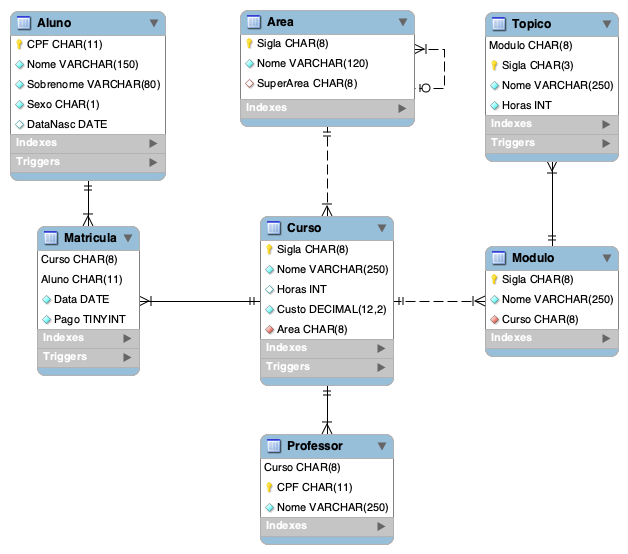
\includegraphics[scale=.6]{images/SAM-EER.png}
\end{center}
\caption{EER do modelo de implementa\c{c}\~ao relacional do SAM (v1.0)}
\label{fig:eer2}
\end{figure}

%Alguns aspectos do projeto l\'ogico n\~ao podem ser captados diretamente pelos diagramas. Diante disso, o Anexo~\ref{sec:anexo1} desse relat\'orio apresenta o \textit{script} para defini\c{c}\~ao do banco de dados com as restri\c{c}\~oes b\'asicas j\'a apresentadas nos diagramas das figuras~\ref{fig:eer} e~\ref{fig:eer2}, al\'em de outras restri\c{c}\~oes ocultas nesses diagramas.

\clearpage
%\section{Projeto F\'isico}
%\label{sec:projetofisico}
%
%\begin{itemize}
%    \item Pedro Martins has already written a tutorial specifically for linguists that also happens to be the best beginner-oriented \LaTeX{} tutorial that we have ever found. You can find it here: \url{http://ptmartins.info/latex/}.
%    \item Our \href{https://www.overleaf.com/latex/templates/pomona-linguistics-quick-reference-guide/jthrqbrktmrd}{Quick Reference Guide} includes detailed instructions for how to format things for phonology (e.g. SPE rules, derivations, tableaux, etc) as well as for syntax (e.g. trees, interlinear glosses), as well as additional details about general \LaTeX{} formatting. It should have every kind of formatting you need to write a Pomona Linguistics paper.
%    \item Michael Diercks aggregates \LaTeX{} resources useful for LGCS students on \href{http://pages.pomona.edu/~mjd14747/tex.html}{his website}.
%\end{itemize}

\clearpage
\section{Conclus\~ao}
O presente relat\'orio apresentou o projeto do banco de dados SAM (v1.0) para um sistema acad\^emico de matr\'icula que, em sua vers\~ao 1.0, pode ser utilizado por diversas institui\c{c}\~oes de ensino para gerenciar seus processos de matr\'icula de alunos em cursos.
Especificamente, propusemos uma especifica\c{c}\~ao de minimundo e apresentamos os requisitos funcionais e operacionais, o projeto conceitual, l\'ogico e f\'isico do banco de dados, concebido no paradigma relacional e projetado para ser implementado em um SGBD relacional comercial.

\clearpage
\section{Anexos: Scripts de Banco de Dados}
\label{sec:anexos}

%\subsection{\textit{Scripts} de Defini\c{c}\~ao do Banco de Dados}
%\label{sec:anexo1}
%
%Vamos ver
%
%\subsection{\textit{Scripts} de Cria\c{c}\~ao de Tabelas}
%\label{sec:anexo1_tables}

% Vamos ver

\paragraph{\textit{Scripts} de Cria\c{c}\~ao de Tabelas}

\begin{verbatim}
-- MySQL Script generated by MySQL Workbench
-- Wed Apr  8 08:32:55 2020
-- Model: New Model    Version: 1.0
-- MySQL Workbench Forward Engineering

SET @OLD_UNIQUE_CHECKS=@@UNIQUE_CHECKS, UNIQUE_CHECKS=0;
SET @OLD_FOREIGN_KEY_CHECKS=@@FOREIGN_KEY_CHECKS, FOREIGN_KEY_CHECKS=0;
SET @OLD_SQL_MODE=@@SQL_MODE, SQL_MODE='TRADITIONAL,ALLOW_INVALID_DATES';

DROP SCHEMA IF EXISTS `SAM` ;

CREATE SCHEMA IF NOT EXISTS `SAM` DEFAULT CHARACTER SET utf8 ;

USE `SAM` ;

DROP TABLE IF EXISTS `Aluno` ;
DROP TABLE IF EXISTS `Area` ;
DROP TABLE IF EXISTS `Curso` ;
DROP TABLE IF EXISTS `Matricula` ;
DROP TABLE IF EXISTS `Modulo` ;
DROP TABLE IF EXISTS `Professor` ;
DROP TABLE IF EXISTS `Topico` ;

CREATE TABLE IF NOT EXISTS `Aluno` (
  `CPF` CHAR(11) NOT NULL,
  `Nome` VARCHAR(150) NOT NULL,
  `Sobrenome` VARCHAR(80) NOT NULL,
  `Sexo` CHAR(1) NOT NULL,
  `DataNasc` DATE)
ENGINE = InnoDB;

CREATE TABLE IF NOT EXISTS `Area` (
  `Sigla` CHAR(8) NOT NULL,
  `Nome` VARCHAR(120) NOT NULL,
  `SuperArea` CHAR(8) NULL)
ENGINE = InnoDB;

CREATE TABLE IF NOT EXISTS `Curso` (
  `Sigla` CHAR(8) NOT NULL,
  `Nome` VARCHAR(250) NOT NULL,
  `Horas` INT NULL,
  `Custo` DECIMAL(12,2) NOT NULL,
  `Area` CHAR(8) NOT NULL)
ENGINE = InnoDB;

CREATE TABLE IF NOT EXISTS `Matricula` (
  `Curso` CHAR(8) NOT NULL,
  `Aluno` CHAR(11) NOT NULL,
  `Data` DATE NOT NULL,
  `Pago` TINYINT NOT NULL DEFAULT 0)
ENGINE = InnoDB;

CREATE TABLE IF NOT EXISTS `Modulo` (
  `Sigla` CHAR(8) NOT NULL,
  `Nome` VARCHAR(250) NOT NULL,
  `Curso` CHAR(8) NOT NULL)
ENGINE = InnoDB;

CREATE TABLE IF NOT EXISTS `Professor` (
  `Curso` CHAR(8) NOT NULL,
  `CPF` CHAR(11) NOT NULL,
  `Nome` VARCHAR(250) NOT NULL)
ENGINE = InnoDB;

CREATE TABLE IF NOT EXISTS `Topico` (
  `Modulo` CHAR(8) NOT NULL,
  `Sigla` CHAR(3) NOT NULL,
  `Nome` VARCHAR(250) NOT NULL,
  `Horas` INT NOT NULL)
ENGINE = InnoDB;

SET SQL_MODE=@OLD_SQL_MODE;
SET FOREIGN_KEY_CHECKS=@OLD_FOREIGN_KEY_CHECKS;
SET UNIQUE_CHECKS=@OLD_UNIQUE_CHECKS;

\end{verbatim}

\paragraph{\textit{Scripts} de Cria\c{c}\~ao de Restri\c{c}\~oes}

%\subsubsection{\textit{Scripts} de Cria\c{c}\~ao de Restri\c{c}\~oes}
%\label{sec:anexo1_constraints}
%
\begin{verbatim}
-- MySQL Script generated by MySQL Workbench
-- Wed Apr  8 08:32:55 2020
-- Model: New Model    Version: 1.0
-- MySQL Workbench Forward Engineering

SET @OLD_UNIQUE_CHECKS=@@UNIQUE_CHECKS, UNIQUE_CHECKS=0;
SET @OLD_FOREIGN_KEY_CHECKS=@@FOREIGN_KEY_CHECKS, FOREIGN_KEY_CHECKS=0;
SET @OLD_SQL_MODE=@@SQL_MODE, SQL_MODE='TRADITIONAL,ALLOW_INVALID_DATES';

USE `SAM`;

ALTER TABLE `Aluno` ADD CONSTRAINT `PK_Curso` PRIMARY KEY (`CPF`);
ALTER TABLE `Area` ADD CONSTRAINT `PK_Area` PRIMARY KEY (`Sigla`);
ALTER TABLE `Curso` ADD CONSTRAINT `PK_Curso` PRIMARY KEY (`Sigla`);
ALTER TABLE `Matricula` ADD CONSTRAINT `PK_Matricula` PRIMARY KEY (`Curso`, `Aluno`);
ALTER TABLE `Modulo` ADD CONSTRAINT `PK_Modulo` PRIMARY KEY (`Sigla`);
ALTER TABLE `Professor` ADD CONSTRAINT `PK_Professor` PRIMARY KEY (`Curso`, `CPF`);
ALTER TABLE `Topico` ADD CONSTRAINT `PK_Topico` PRIMARY KEY (`Modulo`,`Sigla`);

ALTER TABLE `Area` ADD CONSTRAINT `FK_Area_Area`
    FOREIGN KEY (`SuperArea`)
    REFERENCES `Area` (`Sigla`)
    ON DELETE SET NULL
    ON UPDATE CASCADE;

ALTER TABLE `Curso` ADD CONSTRAINT `FK_Curso_Area`
    FOREIGN KEY (`Area`)
    REFERENCES `Area` (`Sigla`)
    ON DELETE RESTRICT
    ON UPDATE CASCADE;

ALTER TABLE `Matricula` ADD CONSTRAINT `FK_Matricula_Curso`
    FOREIGN KEY (`Curso`)
    REFERENCES `Curso` (`Sigla`)
    ON DELETE RESTRICT
    ON UPDATE CASCADE;
ALTER TABLE `Matricula` ADD CONSTRAINT `FK_Matricula_Aluno`
    FOREIGN KEY (`Aluno`)
    REFERENCES `Aluno` (`CPF`)
    ON DELETE CASCADE
    ON UPDATE CASCADE;

ALTER TABLE `Modulo` ADD CONSTRAINT `FK_Modulo_Curso`
    FOREIGN KEY (`Curso`)
    REFERENCES `Curso` (`Sigla`)
    ON DELETE CASCADE
    ON UPDATE CASCADE;

ALTER TABLE `Professor` ADD CONSTRAINT `FK_Professor_Curso`
    FOREIGN KEY (`Curso`)
    REFERENCES `Curso` (`Sigla`)
    ON DELETE CASCADE
    ON UPDATE CASCADE;

ALTER TABLE `Topico` ADD CONSTRAINT `FK_Topico_Modulo`
    FOREIGN KEY (`Modulo`)
    REFERENCES `Modulo` (`Sigla`)
    ON DELETE CASCADE
    ON UPDATE CASCADE;

SET SQL_MODE=@OLD_SQL_MODE;
SET FOREIGN_KEY_CHECKS=@OLD_FOREIGN_KEY_CHECKS;
SET UNIQUE_CHECKS=@OLD_UNIQUE_CHECKS;

\end{verbatim}

\paragraph{\textit{Scripts} de Cria\c{c}\~ao de Restri\c{c}\~oes (Gatilhos)}


%
%\subsubsection{\textit{Scripts} de Cria\c{c}\~ao de Restri\c{c}\~oes (Gatilhos)}
%\label{sec:anexo1_constraints_triggers}
%
\begin{verbatim}

-- MySQL Script generated by MySQL Workbench
-- Wed Apr  8 08:32:55 2020
-- Model: New Model    Version: 1.0
-- MySQL Workbench Forward Engineering

SET @OLD_UNIQUE_CHECKS=@@UNIQUE_CHECKS, UNIQUE_CHECKS=0;
SET @OLD_FOREIGN_KEY_CHECKS=@@FOREIGN_KEY_CHECKS, FOREIGN_KEY_CHECKS=0;
SET @OLD_SQL_MODE=@@SQL_MODE, SQL_MODE='TRADITIONAL,ALLOW_INVALID_DATES';

DELIMITER $$

USE `SAM`$$
DROP TRIGGER IF EXISTS `Aluno_BEFORE_UPDATE` $$
USE `SAM`$$
CREATE DEFINER = CURRENT_USER TRIGGER `SAM`.`Aluno_BEFORE_UPDATE` BEFORE UPDATE ON `Aluno` FOR EACH ROW
BEGIN
  IF NEW.Sexo = 'f' THEN
	SET NEW.Sexo = 'F';
  ELSEIF NEW.Sexo = 'm' THEN
	SET NEW.Sexo = 'M';
  END IF;
  IF NEW.Sexo <> 'F' AND NEW.Sexo <> 'M' THEN
    SIGNAL SQLSTATE '45000'
        SET MESSAGE_TEXT = 'Sexo invalido: F ou M';
  END IF;
END$$

USE `SAM`$$
DROP TRIGGER IF EXISTS `Curso_BEFORE_UPDATE` $$
USE `SAM`$$
CREATE DEFINER = CURRENT_USER TRIGGER `SAM`.`Curso_BEFORE_UPDATE` BEFORE UPDATE ON `Curso` FOR EACH ROW
BEGIN
  IF NEW.Horas < 1 THEN
    SIGNAL SQLSTATE '45000'
        SET MESSAGE_TEXT = 'Horas invalida: Horas > 0';
  END IF;
END$$

USE `SAM`$$
DROP TRIGGER IF EXISTS `Matricula_BEFORE_UPDATE` $$
USE `SAM`$$
CREATE DEFINER = CURRENT_USER TRIGGER `SAM`.`Matricula_BEFORE_UPDATE` BEFORE UPDATE ON `Matricula` FOR EACH ROW
BEGIN
  IF NEW.Pago <> 0 AND NEW.Pago <> 1 THEN
    SIGNAL SQLSTATE '45000'
        SET MESSAGE_TEXT = 'Pago invalido: 0 ou 1';
  END IF;
END$$

USE `SAM`$$
DROP TRIGGER IF EXISTS `Topico_BEFORE_UPDATE` $$
USE `SAM`$$
CREATE DEFINER = CURRENT_USER TRIGGER `SAM`.`Topico_BEFORE_UPDATE` BEFORE UPDATE ON `Topico` FOR EACH ROW
BEGIN
  IF NEW.Horas < 1 THEN
    SIGNAL SQLSTATE '45000'
        SET MESSAGE_TEXT = 'Horas invalida: Horas > 0';
  END IF;
END$$

DELIMITER ;

SET SQL_MODE=@OLD_SQL_MODE;
SET FOREIGN_KEY_CHECKS=@OLD_FOREIGN_KEY_CHECKS;
SET UNIQUE_CHECKS=@OLD_UNIQUE_CHECKS;

\end{verbatim}

\paragraph{\textit{Scripts} de Cria\c{c}\~ao de \'Indices}

%
%\subsubsection{\textit{Scripts} de Cria\c{c}\~ao de \'Indices}
%\label{sec:anexo1_index}
%
\begin{verbatim}
-- MySQL Script generated by MySQL Workbench
-- Wed Apr  8 08:32:55 2020
-- Model: New Model    Version: 1.0
-- MySQL Workbench Forward Engineering

SET @OLD_UNIQUE_CHECKS=@@UNIQUE_CHECKS, UNIQUE_CHECKS=0;
SET @OLD_FOREIGN_KEY_CHECKS=@@FOREIGN_KEY_CHECKS, FOREIGN_KEY_CHECKS=0;
SET @OLD_SQL_MODE=@@SQL_MODE, SQL_MODE='TRADITIONAL,ALLOW_INVALID_DATES';

USE `SAM`;

CREATE UNIQUE INDEX `UN_Area_Nome` ON `Area` (`Nome` ASC);
CREATE INDEX `IDX_FK_Area_Area` ON `Area` (`SuperArea` ASC);

CREATE INDEX `IDX_FK_Curso_Area` ON `Curso` (`Area` ASC);

CREATE INDEX `IDX_FK_Matricula_Aluno` ON `Matricula` (`Aluno` ASC);

CREATE INDEX `IDX_FK_Modulo_Curso` ON `Modulo` (`Curso` ASC);

CREATE INDEX `IDX_FK_Professor_Curso` ON `Professor` (`Curso` ASC);

CREATE INDEX `IDX_FK_Topico_Modulo` ON `Topico` (`Modulo` ASC);

SET SQL_MODE=@OLD_SQL_MODE;
SET FOREIGN_KEY_CHECKS=@OLD_FOREIGN_KEY_CHECKS;
SET UNIQUE_CHECKS=@OLD_UNIQUE_CHECKS;

\end{verbatim}

\paragraph{\textit{Scripts} de Cria\c{c}\~ao do Banco de Dados}

%
%\subsection{\textit{Scripts} de Cria\c{c}\~ao do Banco de Dados}
%\label{sec:anexo2}
%
\begin{verbatim}

USE `SAM` ;

INSERT INTO `Aluno` VALUES ('00506238866','Lisette','Friesen','F','2006-11-30'),
('00694710542','Lorine','Willms','F','2019-09-14'),
('01389490385','Orie','Daugherty','F','1986-10-25'),
('01525324976','Cali','Haag','F','1998-12-12'),
('01586644848','Jackeline','Barton','F','1994-08-16');

INSERT INTO `Area` (`Sigla`, `Nome`, `SuperArea`) VALUES ('10000003', 'Ciências Exatas e da Terra',NULL);
INSERT INTO `Area` (`Sigla`, `Nome`, `SuperArea`) VALUES ('20000006', 'Ciências Biológicas',NULL);
INSERT INTO `Area` (`Sigla`, `Nome`, `SuperArea`) VALUES ('30000009', 'Engenharias',NULL);
INSERT INTO `Area` (`Sigla`, `Nome`, `SuperArea`) VALUES ('40000001', 'Ciências da Saúde',NULL);
INSERT INTO `Area` (`Sigla`, `Nome`, `SuperArea`) VALUES ('50000004', 'Ciências Agrárias',NULL);
INSERT INTO `Area` (`Sigla`, `Nome`, `SuperArea`) VALUES ('60000007', 'Ciências Sociais Aplicadas',NULL);
INSERT INTO `Area` (`Sigla`, `Nome`, `SuperArea`) VALUES ('70000000', 'Ciências Humanas',NULL);
INSERT INTO `Area` (`Sigla`, `Nome`, `SuperArea`) VALUES ('80000002', 'Lingüística, Letras e Artes',NULL);
INSERT INTO `Area` (`Sigla`, `Nome`, `SuperArea`) VALUES ('90000005', 'Outra',NULL);
INSERT INTO `Area` (`Sigla`, `Nome`, `SuperArea`) VALUES ('10100008', 'Matemática','10000003');
INSERT INTO `Area` (`Sigla`, `Nome`, `SuperArea`) VALUES ('10200002', 'Probabilidade e Estatística','10000003');
INSERT INTO `Area` (`Sigla`, `Nome`, `SuperArea`) VALUES ('10300007', 'Ciência da Computação','10000003');
INSERT INTO `Area` (`Sigla`, `Nome`, `SuperArea`) VALUES ('10400001', 'Astronomia','10000003');
INSERT INTO `Area` (`Sigla`, `Nome`, `SuperArea`) VALUES ('10500006', 'Física','10000003');

INSERT INTO Curso (`Sigla`, `Nome`, `Horas`,`Custo`,`Area`) VALUES ('10101012', 'Conjuntos', 1143, 3242.00, '10101004');
INSERT INTO Curso (`Sigla`, `Nome`, `Horas`,`Custo`,`Area`) VALUES ('10101020', 'Lógica Matemática', 4255, 18112.00, '10101004');
INSERT INTO Curso (`Sigla`, `Nome`, `Horas`,`Custo`,`Area`) VALUES ('10101039', 'Teoria dos Números', 2572, 199563.00, '10101004');
INSERT INTO Curso (`Sigla`, `Nome`, `Horas`,`Custo`,`Area`) VALUES ('10101047', 'Grupos de Álgebra Não-Comutaviva', 2481, 185295.00, '10101004');
INSERT INTO Curso (`Sigla`, `Nome`, `Horas`,`Custo`,`Area`) VALUES ('10101055', 'Álgebra Comutativa', 2795, 478753.00, '10101004');
INSERT INTO Curso (`Sigla`, `Nome`, `Horas`,`Custo`,`Area`) VALUES ('10101063', 'Geometria Algébrica', 3670, 64135.00, '10101004');
\end{verbatim}



%
%\subsection{Useful commands for text formatting, some that we built for you}
%
%\ea
%	\begin{tabular}[t]{l l l}
%		\toprule
%		\textbf{Symbol/Annotation} & \textbf{Example} & \textbf{Code} \\ \midrule
%		Ellipsis & \dots & \verb|\dots| \\
%		Subscript & NP\subs{i} & \verb|NP\subs{i}| \\
%		Superscript & NP\supers{i} & \verb|NP\supers{i}|\\
%		Bold & \textbf{bold} & \verb|\textbf{bold}| \\
%		Italic & \textit{italic} & \verb|\textit{italic}| \\
%		Small Caps & \textsc{small caps} & \verb|\textsc{small caps}| \\
%		Strikeout & \sout{strikeout} & \verb|\sout{strikeout}| \\
%		Underline & \underline{underline} & \verb|\underline{underline}| \\
%		circle something in text & \circled{something} & \verb|\circled{something}| \\
%		Highlight something & \hl{something} & \verb|\hl{something}| \\
%		Null & \nothing  & \verb|\nothing|\\
%		Theta & \texttheta & \verb|\texttheta|  \\
%		Phi & \ph & \verb|\ph| \\
%		Hash & \# & \verb|\#| \\
%		Label a left bracket & \Lb{VP} kick it ] & \verb|\Lb{VP}|\\
%		Label a right bracket & [[kick\Rb{rt}ed\Rb{wd} & \verb|\Rb{rt},\Rb{wd}|\\
%		Trace with index & \tr{k}  & \verb|\tr{k}| \\
%		Bar-level node & X\1 & \verb|X\1| \\
%		Head Node & X\0 & \verb|X\0| \\
%		\bottomrule
%	\end{tabular}
%\z
%
%\newpage
%
%\begin{itemize}
%
%\item If you want to make a bulleted list, look at how this list is formatted in the .tex document with the ``itemize'' environment.
%
%\item As you've already seen if you are paying attention to the .tex document on the left of your screen, sections, subsections, and sub-subsection are formatted with the commands \verb|\section{}|, \verb|\subsection{}|, and \verb|\subsubsection{}|, respectively.
%
%\item Look at the .tex document to see how we bolded \textbf{this text} (and Overleaf has a shortcut to make it easy, Cmd-B on Macs, Ctrl-B on PCs). \textit{Similarly for italics}, Overleaf provides a shortcut (Cmd-I on Macs, Ctrl-I on PCs).
%
%\item Write footnotes like this.\footnote{Hey, I'm a footnote.}
%
%\end{itemize}
%
%\subsection{Numbered examples}
%
%\ea
%Numbered examples look like this.
%\z
%
%\noindent Interlinear glossing can be seen in (\ref{BukusuNegation}), which also illustrates cross-references as well.
%
%\ea \label{BukusuNegation}
%\gll Peter se-a-la-ba a-kula sitabu ta. \hspace{2 in}  \textbf{Lubukusu} \\
%Peter NEG-SA-TNS-be SA-buy book NEG \\
%\glt `Peter will not be buying a book.'
%\z
%
%%See the Quick Reference Guide for more detailed instructions on numbered examples, interlinear glossing, and cross-references
%
%\subsection{Tables}
%
%A table is illustrated in (\ref{SampleTable}), though tables can be formatted in many ways (see the Quick Reference Guide).
%
%\ea \label{SampleTable}
%\begin{tabular}[t]{|c|c|c|}
%\hline
%\textbf{Header 1} & \textbf{Header 2} & \textbf{Header 3} \\
%\hline\hline
%cell 1 & cell 2 & cell 3 \\
%\hline
%cell 4 & cell 5 & cell 6 \\
%\hline
%cell 7 & cell 8 & cell 9 \\
%\hline
%\end{tabular}
%
%\z



\end{document}
